\chapter{Introduction}
\label{sec:intro}

Machine Learning and Deep Learning approaches require usually a large amount of simulation
or experimental data which might not be always feasible to obtain due to the complexity
of the simulations and the expensiveness of the experiments. Presence of the limited data often
causes data-driven approaches to fail to deliver adequate accuracy since they are purely
data-dependent. Thus, the data-driven methods with non-matching
real-world observations (sensor or experimental data) or wrong labeled datasets are
prone mostly to make the wrong predictions, which can lead the irrevocable failures 
as there is no physics-based control mechanism to validate the predictions. To compensate
for the lack of adequate data and unknown black-box behavior of the data-driven approaches,
Raissi et al. proposed an approach that combines the data-driven methods
with the existing physics knowledge of the given problem \cite{raissi2019physics}. With this approach,
the data-driven method can learn even with less data since the governing equations of the 
problem are involved in the learning process.    

\hspace{1cm}

As depicted in Figure \ref{fig:data_physics}, obtaining more data is more expensive 
due to the need for more simulation or experiments, while involving more physics increases 
the complexity of the problem. Herein, physics-informed neural networks (PINNs) come 
into play, which requires some data and some physics. PINNs enforce the neural network architecture
to learn the pattern by using the limited data with the help of the governing equations of 
the problem \cite{kollmannsbergerdeep}. 

\hspace{1cm}

\begin{figure}[thbp]
    \centering
    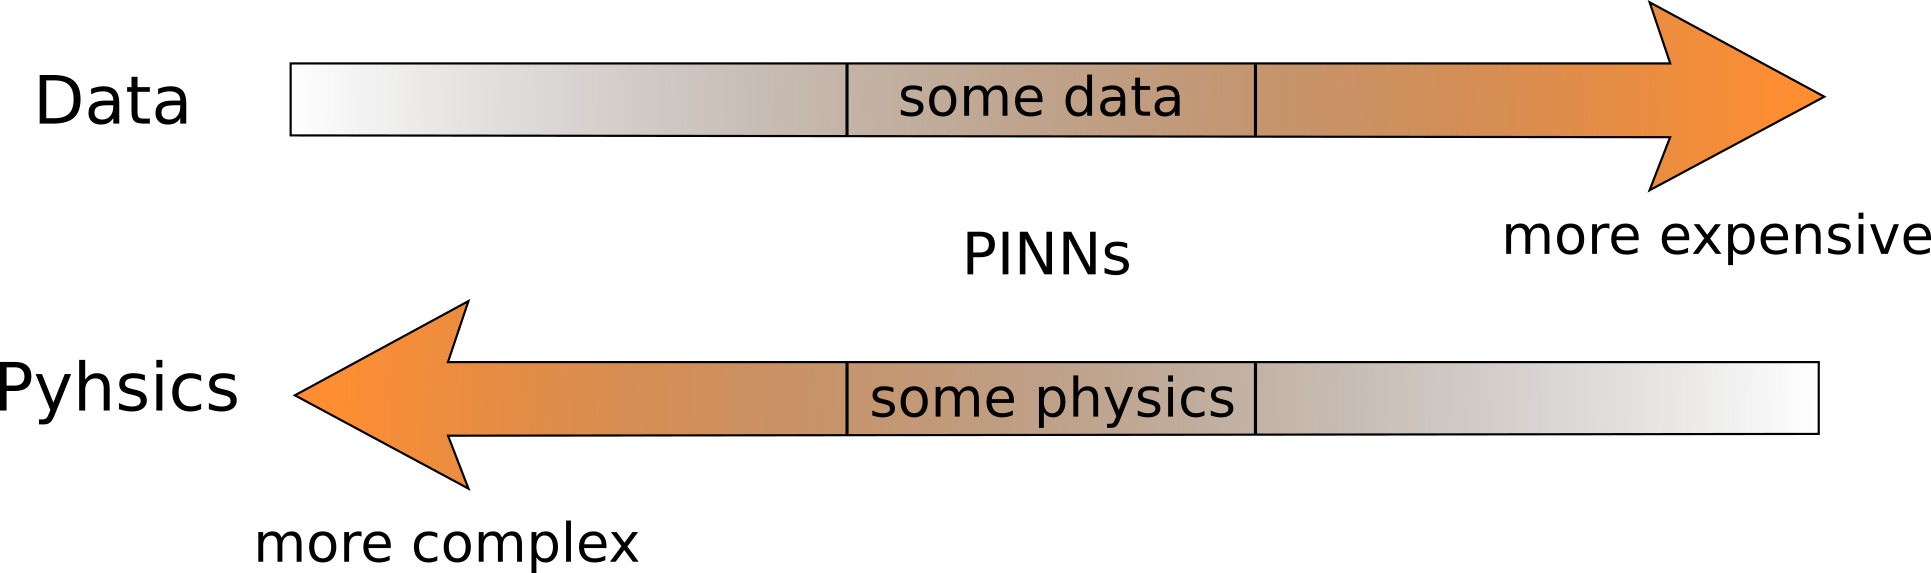
\includegraphics[scale=0.55]{data_physics.png}  
    \caption{Trade-off between data and physics}
    \label{fig:data_physics}
\end{figure}

